\chapter{Reconstruction} % 

The precise measurement of particles produced in the high energy collisions at the LHC 
is necessary to effectively execute the CMS physics programme. This requires high precision
reconstruction and identification of physics objects in a challenging environment containing
large numbers of different particles with a range of energies. The \alphat analysis 
relies directly on reconstruction of jets and \met for the signal region and on the 
reconstruction of leptons and photons to reject electroweak 
backgrounds and to define control regions.
This requires the use of information from all detector subsystems and state-of-the-art
techniques to allow the reconstruction, selection and calibration of these physics objects.


\section{Detector reconstruction}

The first stage in reconstructing the physics objects is to produce the necessary
input information from the detector subsystems. This takes the form of both the tracks, 
trajectories, of charged particles as well as the energy measurements from
calorimeter depositions. Specialist algorithms which suppress backgrounds, 
mitigate the effects of pileup and provide high resolution energy,
position and/or temporal measurements are used to optimise the precision of the 
measured quantities over a wide range of particle energies and momenta.

\subsection{Track reconstruction}

Charged particle tracks are reconstructed from the hits, considering the efficiency and resolution, 
using the iterative Combinatorial Track Finder (CTF) algorithm. The track reconstruction can be decomposed 
into four logical steps outlined below.

\begin{itemize}
\item Seeds are generated using either triplets of tracker hits or pairs of hits with an additional constraint 
from the beamspot or a pixel vertex. This gives an initial estimate of the trajectory with uncertainty \cite{tracker_early}.
\item Each seed is propagated outward through the tracker layers considering the current uncertainty in the trajectory.
In propagating, a uniform magnetic field as well as no energy loss or multiple Coulomb scattering effects are assumed.
The track parameters are updated with the best matching hit on each layer (if any) according to the Kalman filter formalism \cite{tracker_vertex}.
The search continues until either the boundary of the tracker is reached or no more compatible hits are found. If a minimum number
of valid hits are observed an inwards search is initiated for additional hits\cite{tracker_early}.
\item It is possible for a single charged particle track to be reconstructed more than once, starting either from different seeds or if
one seed develops into multiple track candidates. If the fraction of shared hits between two track candidates is greater
than 19\% (determined empirically) the track with fewer hits is discarded. If the number of hits is equivalent the track with
 the largest $\chi^2$ is discarded\cite{tracker_vertex}.
\item After the track candidates are built and cleaned the hits in each candidate are refitted using a Kalman filter and smoother. This 
avoids possible bias from the seeding stage \cite{tracker_vertex}.
\end{itemize}

The CTF performs six iterations to determine the tracks. Between each iteration any hits that are assigned to tracks in the
previous iteration are removed from the collection. The final track collection is then filtered to remove fake tracks using 
information on the number of hits, the $\chi^2$ and the compatibility of the track originating from a pixel vertex. The momentum 
resolution achieved is 0.7 (5)\% at 1 (1000) \GeV in the central region\cite{tracker_early}. Using a dataset of pions and muons from an early run 
at the LHC the tracking efficiency was measured as 98\% for tracks with $p_T > 500\MeV$ and $>99\%$ for tracks with $p_T > 2\GeV$\cite{tracker_eff}.

\subsection{Vertex Reconstruction}

As described in Sec.~\ref{lhc_intro}, the LHC produced an average of 25 simultaneous collisions per bunch crossing
during Run 2. It is essential to identify the Primary Vertex (PV) and the particles originating from it to allow 
particles from additional collisions to be rejected and to identify features such as displaced vertices. The tracks
are initially clustered using a deterministic annealing (DA) algorithm based on the points of closest approach of the 
tracks to the beamspot \cite{tracker_vertex}. The candidate vertices containing at least two tracks are then
fitted using an adaptive vertex fitter (AVF) to compute the best estimates of vertex parameters \cite{tracker_avf}. 
Each track in the vertex is assigned a weight between 0 and 1 corresponding to the likelihood that that track
belongs to the vertex. The tracks with weight near 1 are most consistent with the reconstructed vertex while
those that are least consistent have small weights. The number of degrees in the fit, defined as 

\begin{equation}
n_{dof} = -3 + 2 \sum_{i=1}^{\#tracks} wi,
\end{equation}

is an important parameter for distinguishing real proton-proton interactions from misclustered vertices as it is strongly corrected with
the number of tracks compatible with arising from the interaction region \cite{tracker_vertex}. The vertex
position and resolution determined using the AVF have been 
measured in early LHC data and compared with simulation as shown in Fig~\ref{fig:pvEffRes}.

\begin{figure}[hbt]
  \begin{center} 
   \subfigure[\label{fig:pvEff}]{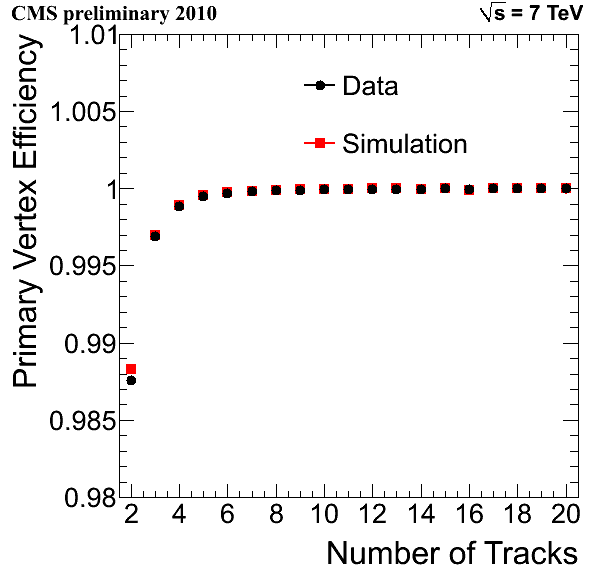
\includegraphics[width=0.5\textwidth]{Figures/detector/pvEff}}~
   \subfigure[\label{fig:pvRes}]{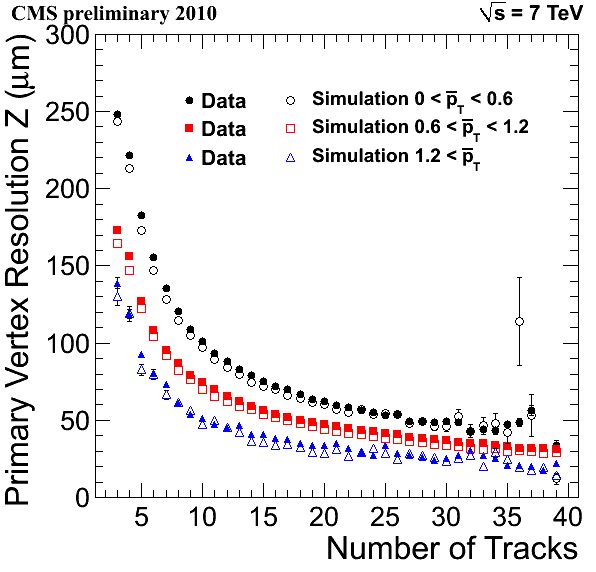
\includegraphics[width=0.5\textwidth]{Figures/detector/pvRes}}
   \caption{(a) Primary Vertex efficiency as a function of the number of associated tracks. (b) Primary Vertex 
   resolution in the z coordinate as a function of the number of associated tracks for three track $p_T$ scenarios \cite{tracker_seven}
   \label{fig:pvEffRes} }
  \end{center}
\end{figure}

The vertices are ordered according to the sum of the $p_T^2$ of the tracks associated to each vertex with the 
vertex with the highest $p_T^2$ taken as the primary vertex (PV). The position of the primary vertex can
be used for object identification and control of pile-up. Many CMS analyses, including the one in this 
thesis, make requirements that a good vertex is reconstructed from the tracks satisfying:

\begin{itemize}
\item A minimum number of degrees of freedom: $n_{dof} > 4$.
\item The collision to occur with $|z| < 24cm$ such that the primary vertex is near the interaction point in the longitudinal direction.
\item The collision to occur within a radial distance of $|d_{xy}| < 24cm$ from the beamline.
\end{itemize}

\subsection{Calorimeter reconstruction}

The calorimeters must reconstruct the energies of incident particles from the energy deposits made in the 
various subsystems. These deposits must be clustered and the measurement calibrated to provide 
details of the energy, position and timing of the incident particle. These can be used to complement 
the information from the tracker and provides necessary redundancy in the case of track
misreconstruction. For neutral particles the calorimeter subsystems provide the only measurement of
the particle properties.

The ECAL crystals are calibrated with both absolute and relative calibrations. Nine EB superclusters
and 500 EE crystals are calibrated using high energy electron beams to achieve a resolution of 0.5\% (1\%) for the EB (EE) components. 
The remainder undergo relative intercalibration to achieve a resolution of 1.4\%-1.8\% ($\sim5\%$) for the EB (EE) components. 
During running the response of the crystals changes due to radiation induced crystal-lattice defects which absorb the scintillation light. 
The crystal transparency is monitored to allow the impact on energy measurements to be assessed and corrected \cite{ecal_calib}. 
The HCAL components undergo a similar calibration to the ECAL crystals. Firstly a subset of the components are calibrated with
a 50 \GeV~pion beam and this is then extended to the remainder of the subsystem using a Co source \cite{hcal_beam}. Additional corrections
for the HCAL component are derived during LHC running \cite{hcal_calib}.

The reconstruction of the energy at the HCAL and ECAL relies on recording the amplified light pulses from the photodiodes over a 25ns time
sample. When operating with 25ns bunch spacing particle energies from previous or following bunch crossings can be integrated
into this sample, biasing the energy measurement. This effect is correcting by using a dedicated reconstruction that removes
the contributions from such Out Of Time Pileup (OOTPU)~\cite{hcal_timing,ecal_timing}. The 25ns sample is fitted including three pulse shape templates with
variable amplitude and arrival times with the central pulse corresponding to the triggered event. The timing distribution for
the ECAL hits above 1~\GeV, which is derived independently from the energy measurement, is shown in Figure~\ref{fig:timing_barrel_linear} showing that
contributions from OOTPU are rejected.

\begin{figure}
\centering
    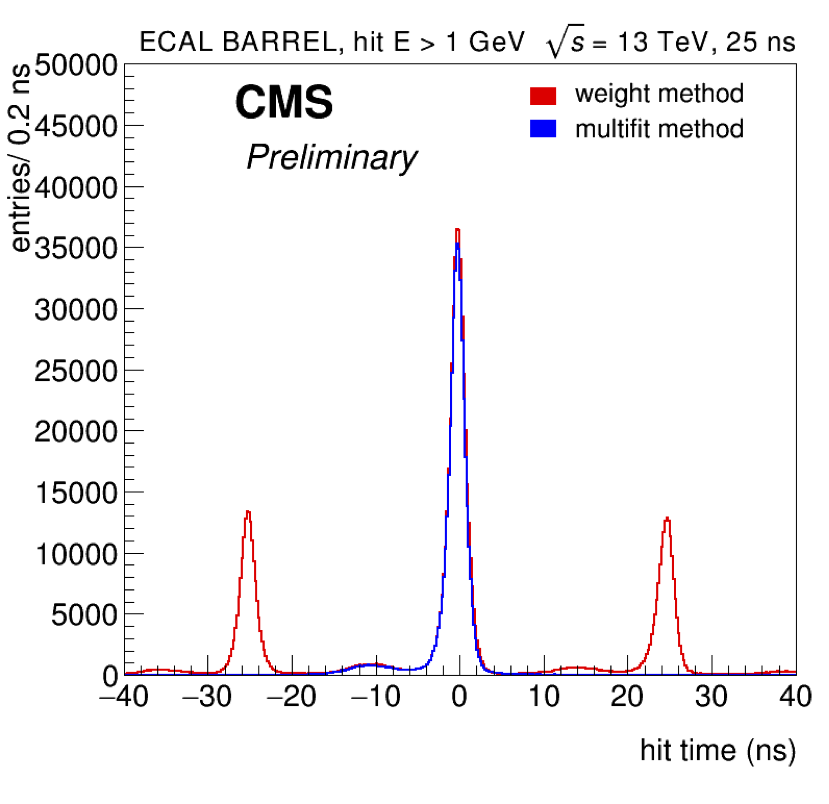
\includegraphics[width=0.8\textwidth]{./Figures/reconstruction/timing_barrel_linear.png}
  \caption{Timing distribution of the hits in the ECAL barrel with a reconstructed energy above 1\GeV~\cite{ecal_timing}.}
  \label{fig:timing_barrel_linear}
\end{figure}

\section{Physics object reconstruction}

The reconstructed tracks and calorimeters form the inputs to the reconstruction of the particles and 
jets that form the basis of the final selection of many analyses, including the analysis described 
in the thesis, referred to as physics objects. These are reconstructed using a combination of
dedicated local reconstruction algorithms as well as the global event Particle Flow algorithm, described in ??.
In addition, several WPs of selection criteria are defined for each physics object 
which provide a range of efficiencies and corresponding proportion of false positives. 

\subsection{Electron and photon reconstruction}

Photons and electrons interact similarly within the ECAL and so these objects follow similar reconstruction techniques.
Electrons are reconstructed by matching information in the tracker and ECAL
using two complementary techniques, an ECAL driven reconstruction described in this section (identical aside from tracking requirements
to the photon reconstruction) and a tracker-driven reconstruction performed with the PF algorithm described in section ??
which is optimal for low $p_T$ electrons. 

In the ECAL, both electron and photon candidates are formed by clustering energy deposits
from electromagnetic showers. Around 50\% of the photons convert into an electron-positron pair in the material proceeding the calorimeter
leaving an energy deposit that is widely spread in $\eta$ and $\phi$ \cite{electron_photon_reco}. 
For unconverted photons the deposits are fairly localised in $\eta$ and $\phi$. Electrons radiate
bremsstrahlung in the presence of the magnetic field and lose $33\%$ of their energy on average
in the central region and up to $86\%$ at $|\eta| = 1.4$. Their energy deposits are widely spread
in $\phi$ but narrow in $\eta$. The hybrid (multi) clustering algorithm exploits this characteristic to
reconstruct high energy electrons and photons in the barrel (endcap). The hybrid algorithm
uses a seed crystal and clusters up to ten strips (dominoes) of $1\times3$ or $1\times5$ ($\phi\times\eta$) within 
$\Delta\phi < 0.3$ from the seed. Any domino with an energy under $100\MeV$ ~is discarded. The dominoes
are themselves clustered in $\phi$ provided each disconnected subcluster has a seed domino of energy $>350\MeV$.
The combination of these subclusters is referred to as a supercluster. The multi reconstruction in the endcap 
follows a similar procedure using $5\times5$ grids of crystals. 

Superclusters which can be associated to tracks originating from the primary vertex are reconstructed as electrons.
As electrons lose energy through the non-Gaussian bremsstrahlung process the Kalman filter is innapropriate and
so the specialist track reconstruction Gaussian Sum Filter algorithm is used. This allows the total energy of
electrons to be reconstructed including the component lost through bremsstrahlung. The photons are identified 
through inverting the track matching criteria of the supercluster. In the endcaps, additional information
is used from the preshower when reconstructing the energy.

Additional selections are applied on all reconstructed electrons and photons to suppress backgrounds.
For electrons these are mainly composed of misreconstructed jets, secondary electrons from photon
conversions and semi-leptonic decays of heavy quarks. As electrons are mainly contained within 
the ECAL a requirement on the ratio of energies in the ECAL and HCAL provides a strong veto of hadronic
backgrounds. In addition, requirements are made on the matching track such that the transverse distance from 
the primary vertex is $d_{xy} < 0.0261$ ($d_{xy} < 0.118$) and the longitudinal distance is $d_z < 0.041$
($d_z < 0.822$) for the barrel (endcap). Several variables that rely on the shower shape and cluster
width are used to reject fakes including the $\sigma_{i\eta i\eta}$ which is the second moment of the log-weighted
distribution of crystal energies calculated in the $5\times5$ matrix around the most energetic crystal. The value of
 $\sigma_{i\eta i\eta}$ is larger on average for neutral meson decay to two collimated photons.

\subsection{Muon reconstruction}

Muons are MIPs, leaving minimal energy deposits in the calorimetry subsystems, and travelling through
the entire detector. The muons are therefore reconstructed using a combination of the inner tracker
and muon systems. Two algorithms are used to give complementary efficiency across the momentum spectrum,
the 'the outside-in' global muon algorithm described in and 'the inside-out' tracker 
muon algorithm described below.

The outside-in algorithm begins with identifying a tracker match for each muon track. Hits in muon
chambers are used to define standalone-muon tracks. These are then matched with tracker tracks
by comparing parameters of the two tracks propagated onto a common surface. The hits from
both systems are then combined and a global muon fit is performed using a Kalman filter. The momentum 
resolution is significantly improved by the global fit over a tracker only fit for muons of $p_T < 200\GeV$ 

The inside-out algorithm selects all tracks satisfying $p_T > 0.5\GeV$ and $p > 2.5\GeV$. These are then 
extrapolated to the muon system taking into account effects from the magnetic field, multiple Coulomb scatting
in the detector material and the average expected energy loses. If at least one muon segment matches 
the extrapolated track the track qualifies as a Tracker Muon. Tracker Muon reconstruction is more efficient
than global muon reconstruction for low momenta of $\sim p< 5\GeV$. This is due to only requiring one segment
of the muon system while global muon reconstruction is more efficient for higher energy muons which are likely
to pass through several muon stations.

In order to ensure the muons are prompt (produced in by the hard process such as vector boson decay) rather
than non-prompt (produced from the in-flight decays of hadrons, taus or heavy quarks) and to reject fakes
caused by the punch through of hadronic particles, additional selections are made. These include quality
selection on the $\chi^2$ of the muon track, a minimum number of valid hits as well as requirements
on distances from the primary vertex $d_{xy} < 0.05 cm$ and $d_{z} < 0.1 cm$ aimed at ensuring prompt muons.

Muons must be reconstructed through either the Global or Tracker Muon algorithm. In combination, and
including additional selections, these provide an efficiency of $>95\%$ for
reconstructing a muon with $p_T$ larger than a few \GeV~over the full $\eta$ range covered by the
muon system and a fake rate from hadrons of $<1\%$.




